% 80-13(인쇄 80쪽) — 한 변의 길이가 1인 정삼각형 ABC 와 변 위를 움직이는 점 P(출발점은 꼭짓점 A).
% C 에서 B 로 가는 점선 호와 그 옆의 1 은 「한 변만큼(=1) 움직인다」를 보인 원문 표시 그대로.
% 스캔 화질이 낮아 TikZ 로 다시 그림(점은 원문대로 A 자리 하나 · 라벨은 원문에 있는 A, B, C, P, 1 뿐 · 확률은 적지 않는다).
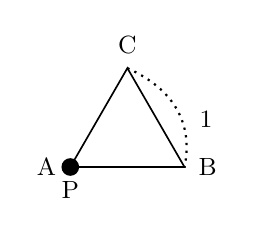
\begin{tikzpicture}[scale=1.45, line width=0.6pt]
  \coordinate (A) at (0,0);
  \coordinate (B) at (1,0);
  \coordinate (C) at (0.5,0.866);
  \draw (A) -- (B) -- (C) -- cycle;
  \fill (A) circle (2.2pt);
  \node[left=1.5pt, font=\small] at (A) {$\mathrm{A}$};
  \node[right=1.5pt, font=\small] at (B) {$\mathrm{B}$};
  \node[above=1.5pt, font=\small] at (C) {$\mathrm{C}$};
  \node[below=1.5pt, font=\small] at (A) {$\mathrm{P}$};
  \draw[dotted, line width=0.8pt] (C) .. controls (1.00,0.64) and (1.06,0.28) .. (B);
  \node[right=1pt, font=\small] at (1.02,0.42) {$1$};
\end{tikzpicture}
